\chapter{Resultados}
\label{chap:resultados}

Este capítulo apresenta uma síntese dos resultados obtidos a partir da execução 
dos \textit{benchmarks} do DaCapo Chopin \cite{dacapochopin}, instrumentada com o JRAPL
\cite{jrapl}. A análise considera a energia do pacote e o tempo de execução,
além das métricas derivadas EDP e \(EDP^2\), que combinam energia e desempenho
em uma mesma medida. Os resultados são apresentados de forma
agregada por frequência do processador e por múltiplos relativos de
\textit{heap}, permitindo observar tendências gerais comuns aos
\textit{benchmarks} avaliados.

\section{Visão geral}

A Figura \ref{fig:summary_heatmaps_serial_gc} apresenta, para cada
\textit{benchmark}, a energia e o tempo normalizados pela melhor configuração
observada para aquele mesmo \textit{benchmark}. Dessa forma, valores próximos de 1 indicam
configurações competitivas, enquanto valores mais altos indicam perda relativa
em comparação com o melhor resultado obtido para o \textit{benchmark}.

\begin{figure}[htbp]
    \centering
    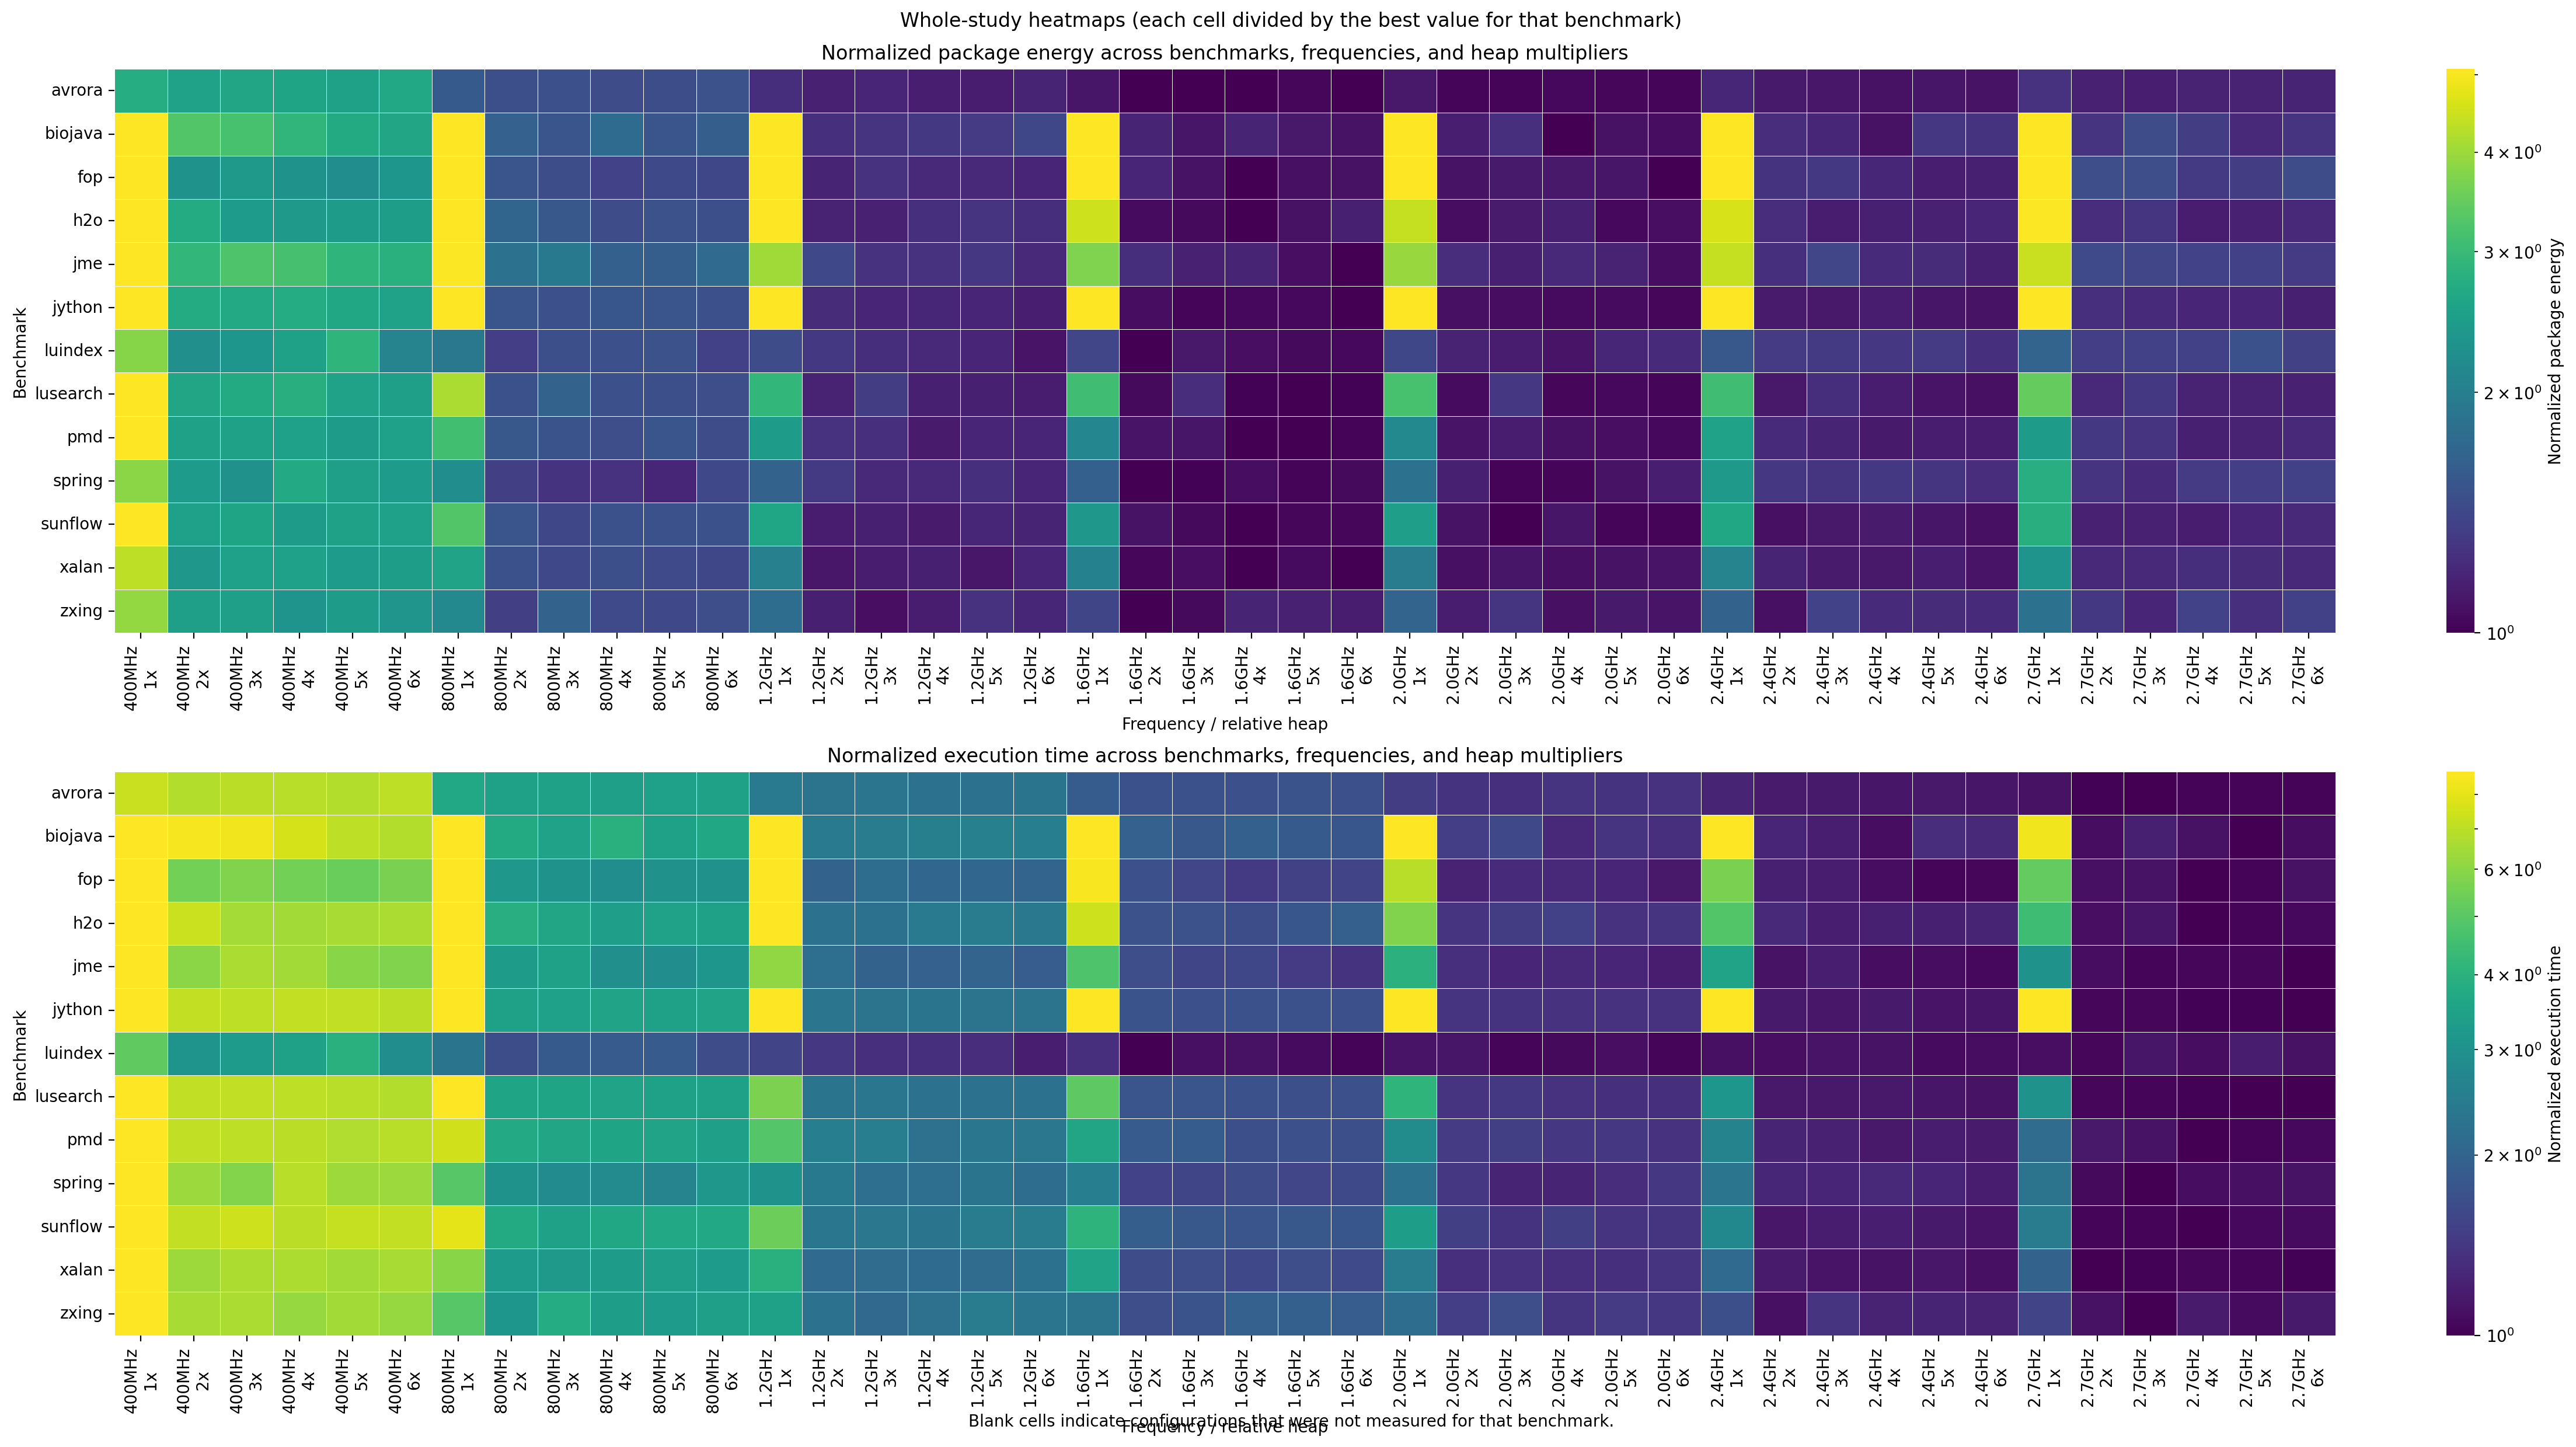
\includegraphics[width=\textwidth]{figs/summary_heatmaps_serial_gc.png}
    \caption{Mapa de calor com energia e tempo normalizados para todos os
    \textit{benchmarks}, frequências e múltiplos de \textit{heap}
    considerados nesta análise.}
    \label{fig:summary_heatmaps_serial_gc}
\end{figure}

Observa-se, inicialmente, que as frequências mais baixas, em especial
400 MHz e 800 MHz, aparecem com frequência fora da região de melhor
desempenho tanto para energia quanto para tempo. Isso indica
que, no conjunto avaliado, faixas de frequência mais baixas do processador
resultam no aumento do tempo de execução em proporção maior do que a eventual 
economia de energia obtida. Isso acontece porque o escalonamento de frequência 
do processador somente afeta a energia consumida pela CPU. A energia consumida 
por outros componentes do sistema não é afetada. Sendo assim, o ganho energético 
obtido com a redução da potência do processador é compensado pelo aumento do 
tempo de execução. Isso mostra as limitações do escalonamento de frequência, 
já que a partir de um certo limite, a diminuição da frequência do processador 
prejudica tanto o tempo de execução quanto a energia consumida \cite{jrapl}.

Por outro lado, as menores energias tendem a se concentrar em frequências
intermediárias, principalmente entre 1{,}6 GHz e 2{,}0 GHz, enquanto os menores
tempos se deslocam para a faixa superior, entre 2{,}4 GHz e 2{,}7 GHz. Essa
separação entre a região de menor consumo energético e a região de melhor
desempenho reforça que minimizar o tempo de execução não é equivalente a
minimizar o consumo de energia, resultado compatível com a discussão de
\citeonline{programming_lang_energy}. O resultado mostra que, para as faixas 
de frequência analisadas, o aumento da frequência do processador quase sempre 
resulta em uma redução no tempo de execução. No entanto, o consumo de energia 
tem uma faixa de frequência ótima, a partir da qual o aumento de frequência 
é prejudicial para o desempenho. Essa divergência reforça a necessidade de 
considerar essas duas métricas no processo de desenvolvimento de \textit{software} 
e pesquisa.

Podemos notar que \textit{heaps} pequenos concentram a maior parte das
configurações menos favoráveis. Considerando os valores normalizados,
a mediana da energia passa de 1{,}677 para 1{,}196 ao se comparar o grupo de
\textit{heaps} de \(2\times\) com o grupo de \textit{heaps} de 
\(3\times\). Para o tempo de execução, a diferença é ainda mais acentuada,
com redução da mediana de 2{,}696 para 1{,}676. Isso indica que o
aumento do espaço de memória disponível para a JVM tende a reduzir tanto a
penalidade energética quanto a penalidade temporal em relação ao melhor caso de
cada \textit{benchmark}. Vale notar que \textit{heaps} muito restritos (próximos 
do mínimo necessário) penalizam fortemente as duas métricas, sendo o fator mais 
relevante no desempenho, já que nem mesmo para as frequências mais altas essa 
configuração de \textit{heap} é competitiva.

\section{Otimização de energia e tempo}

Para complementar a leitura dos mapas de calor, a
Figura \ref{fig:summary_table_serial_gc} mostra quantos \textit{benchmarks}
incluem cada frequência e cada múltiplo de \textit{heap} no conjunto de
configurações estatisticamente empatadas com a melhor média, considerando a
sobreposição dos intervalos de confiança de 95\%. Ou seja, para cada uma dessas 
configurações, a média de energia ou tempo é estatisticamente igual à melhor média 
observada para o \textit{benchmark}. A tabela que mostra as diferentes frequências 
não inclui as frequências de 400MHz e 800MHz, pois nenhum \textit{benchmark} 
apresentou uma configuração com essas frequências que fosse estatisticamente 
igual à melhor média observada.

\begin{figure}[htbp]
    \centering
    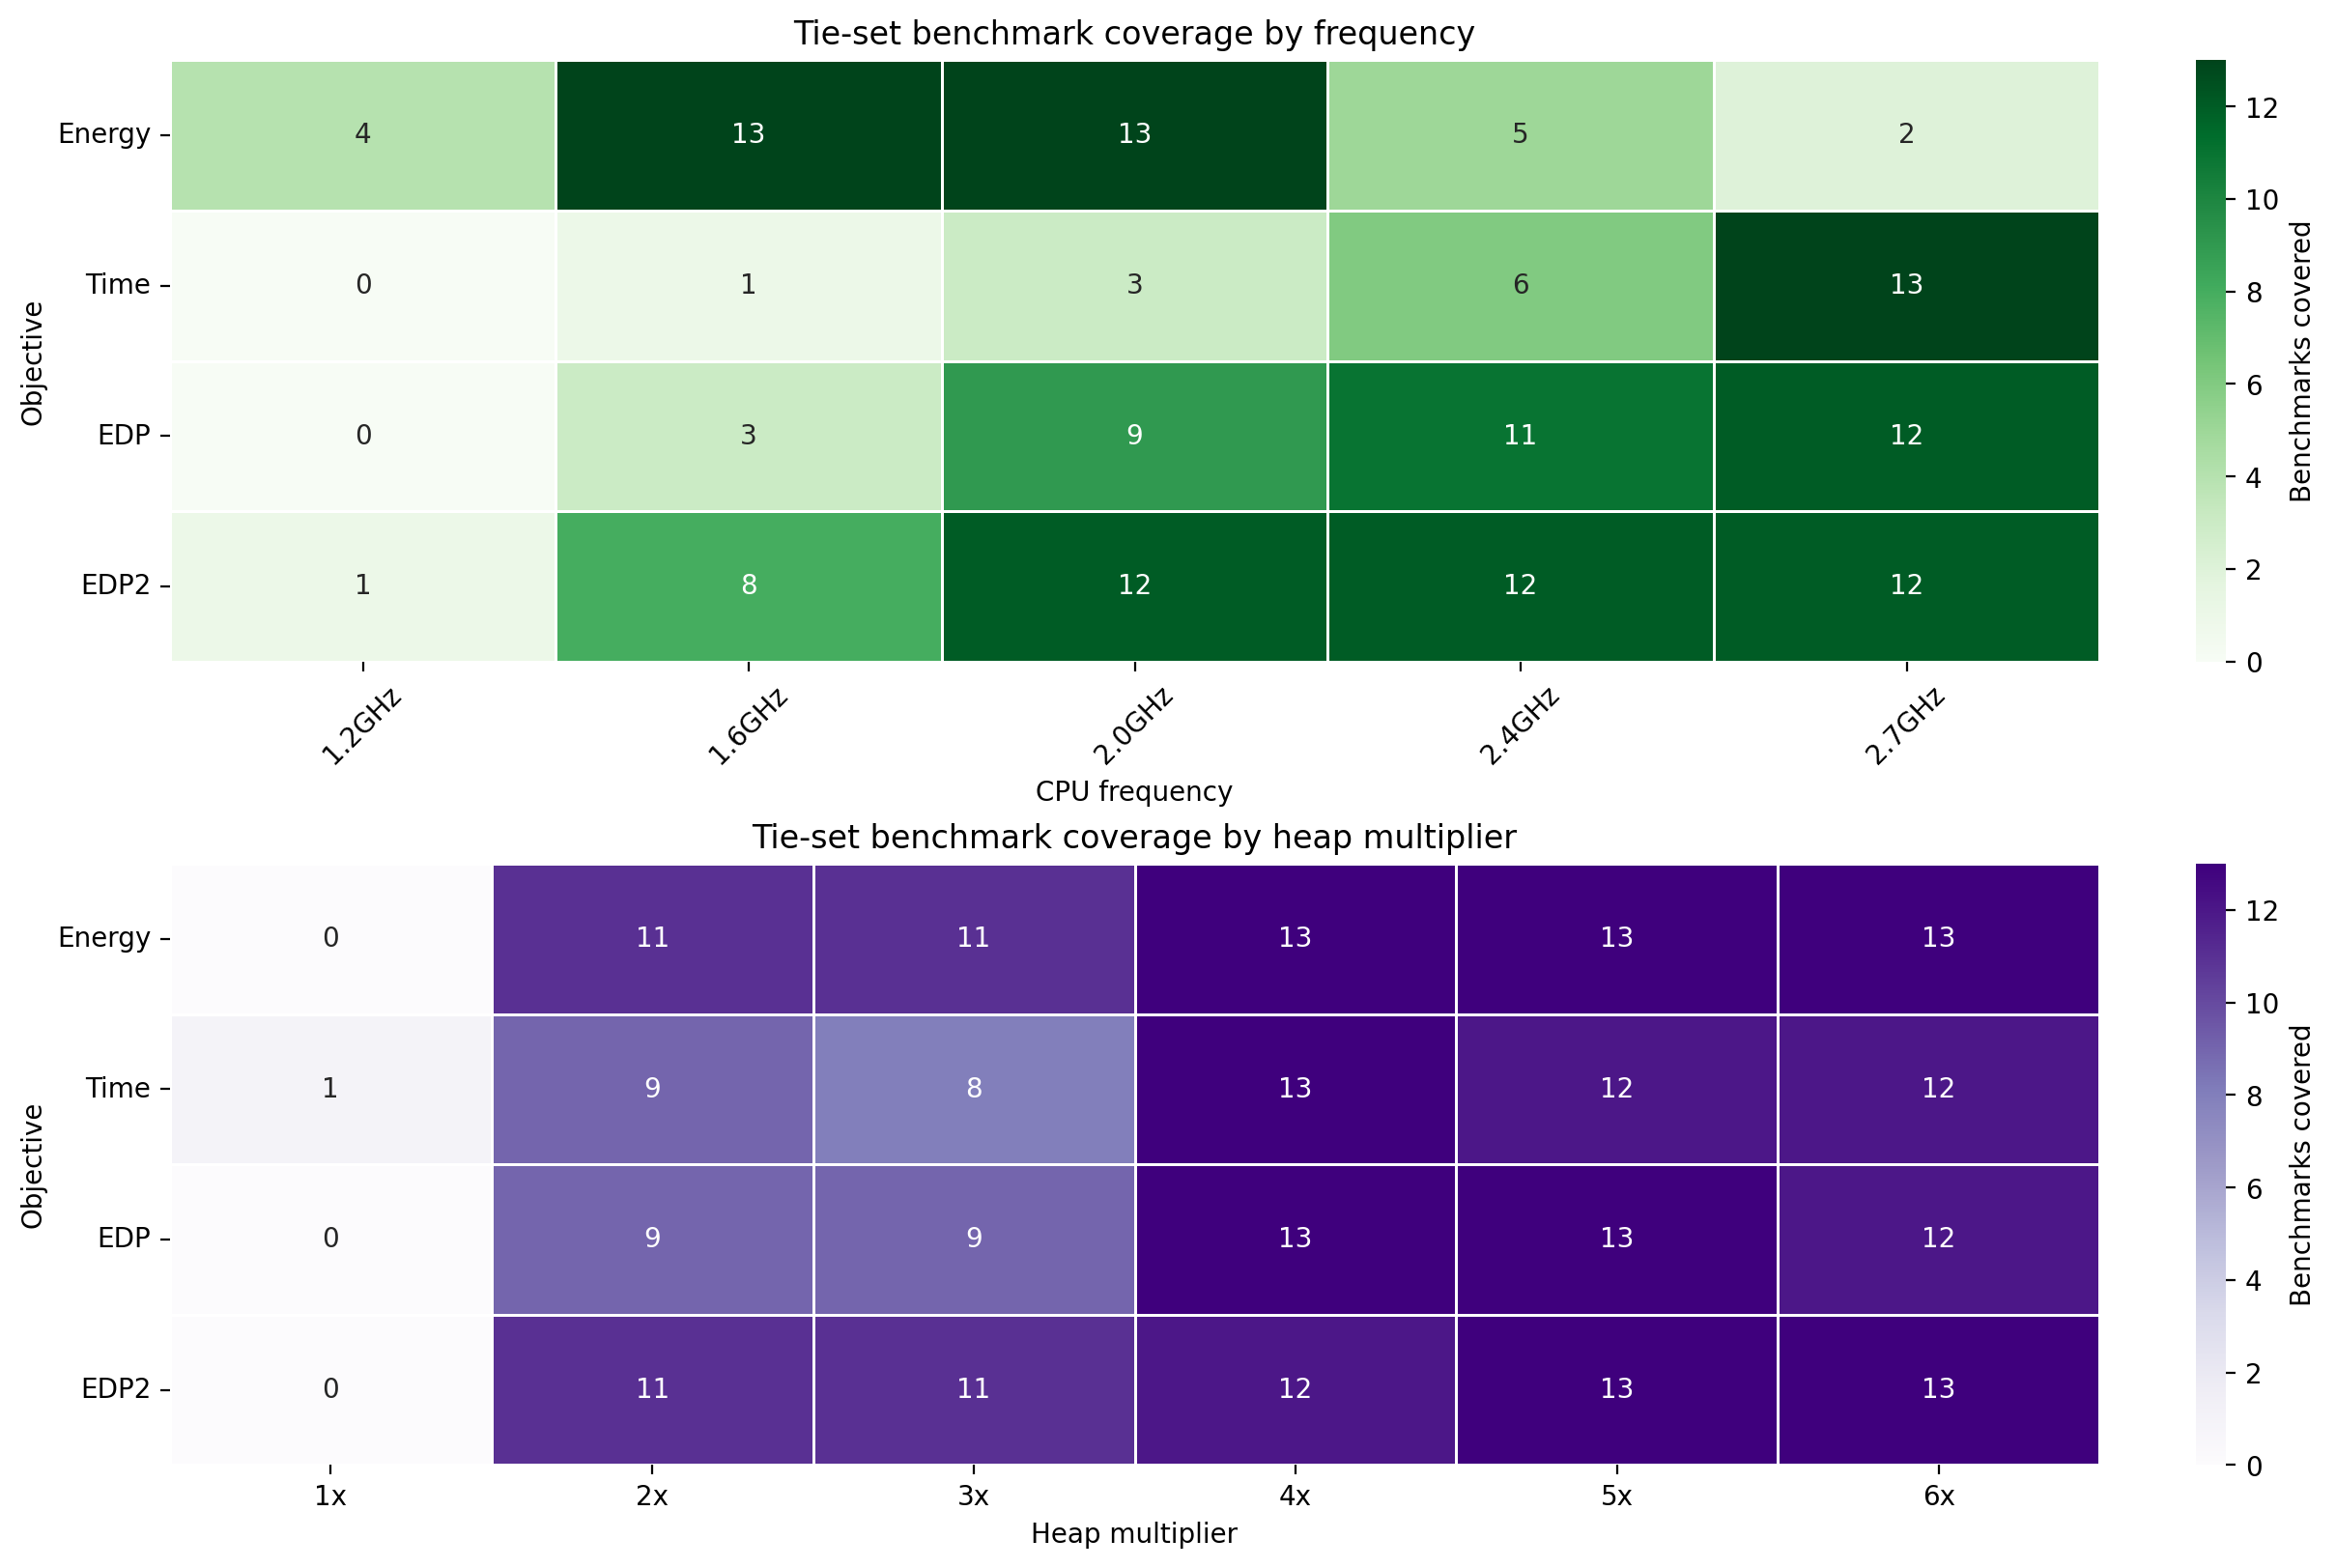
\includegraphics[width=\textwidth]{figs/summary_table_serial_gc.png}
    \caption{Possíveis configurações ótimas para cada \textit{benchmark}, 
    considerando a sobreposição dos intervalos de confiança de 95\%.}
    \label{fig:summary_table_serial_gc}
\end{figure}

Para energia, as frequências de 1{,}6 GHz e 2{,}0 GHz aparecem em 13 dos 13
\textit{benchmarks} analisados, enquanto 2{,}7 GHz aparece em apenas 2. Isso
reforça a interpretação de que a melhor eficiência energética tende a surgir em
frequências intermediárias. Já para tempo, a situação se inverte: 2{,}7 GHz
cobre todos os 13 \textit{benchmarks}, ao passo que frequências menores têm
cobertura muito inferior. Portanto, quando o objetivo principal é otimizar o 
tempo de execução, a tendência predominante é operar próximo da maior frequência 
testada.

Os múltiplos de \textit{heap} apresentam resultados mais similares entre todos 
objetivos testados. Para energia, tempo, EDP e \(EDP^2\), os melhores conjuntos se 
concentram a partir de \(4\times\) o \textit{heap} mínimo, com cobertura de 
12 ou 13 \textit{benchmarks}. Em contraste, o caso de \(1\times\) praticamente 
não aparece nessas regiões e surge apenas uma vez na métrica de tempo. Esse 
resultado sugere que \textit{heaps} mínimos raramente pertencem ao 
conjunto de configurações mais competitivas, enquanto \textit{heaps} maiores 
aparecem com regularidade entre os melhores resultados.

\section{Discussão}

Os dados apresentados mostram que não existe uma configuração ótima
universal para todas as cargas do DaCapo. Alguns \textit{benchmarks}, como
\texttt{jme}, \texttt{zxing}, \texttt{xalan} e \texttt{sunflow}, apresentam
regiões amplas de empate estatístico, indicando que diferentes combinações de
frequência e \textit{heap} produzem resultados semelhantes. Outros, como
\texttt{h2o} e \texttt{jython}, exibem conjuntos mais estreitos, o que sugere
maior sensibilidade às escolhas de configuração.

Outro ponto relevante é que os ótimos de energia e de tempo frequentemente não
coincidem. Entre os 13 \textit{benchmarks} analisados, apenas 6 possuem alguma
sobreposição entre os conjuntos quase ótimos dessas duas métricas. Assim, uma 
política de ajuste voltada exclusivamente para reduzir o tempo de execução 
pode deixar de considerar configurações com consumo energético significativamente 
mais favorável. Ainda sim, há algumas tendências que podem ser observadas 
independentemente do objetivo de otimização. Por exemplo, \textit{heaps} 
mínimos são quase sempre desfavoráveis, recomendando-se no a partir de \(2\times\) 
o mínimo necessário e idealmente a partir de \(4\times\). Isso mostra que ambientes 
com restrições de memória não são os mais adequados para otimização de energia ou tempo. 
Analogamente, frequências muito baixas são desfavoráveis para todos os objetivos 
testados e devem ser evitadas.

Em síntese, os resultados desta análise apontam três tendências principais:
(i) frequências muito baixas são globalmente desfavoráveis; (ii) a energia tende
a ser minimizada em frequências intermediárias, enquanto o tempo favorece as
frequências mais altas; e (iii) \textit{heaps} a partir de \(4\times\) o mínimo 
necessário aparecem de forma recorrente entre as melhores configurações. 
Em conjunto, essas evidências indicam que o comportamento energético da JVM depende 
da interação entre carga de trabalho, frequência do processador e disponibilidade de 
memória, não sendo adequadamente descrito por um único parâmetro de ajuste.